% % % % % % % % % % % % % % % % % % % % % % % % % % % % % % % % % % % % % % %
%
% Copyright (c) 2013 INRA
%
% Gauthier Quesnel - quesnel@users.sourceforge.net
%
% DevLog 2013 - Presentation VLE
%
% Permission is granted to copy, distribute and/or modify this document
% under the terms of the GNU Free Documentation License, Version 1.2
% or any later version published by the Free Software Foundation;
% with no Invariant Sections, no Front-Cover Texts, and no Back-Cover Texts.
% A copy of the license is included in the section entitled "GNU
% Free Documentation License".
%
% % % % % % % % % % % % % % % % % % % % % % % % % % % % % % % % % % % % % % %

\documentclass[xetex, compress, table, svgnames]{beamer}
\usefonttheme[onlymath]{serif}
\usepackage{fontspec}
\usepackage{xltxtra}
\defaultfontfeatures{Ligatures=TeX,Numbers=OldStyle,Scale=MatchLowercase}
\setromanfont[Mapping=tex−text]{Linux Libertine O}
\setsansfont[Mapping=tex−text]{Linux Biolinum O}
\setmonofont[Mapping=tex−text,Scale=0.9]{Courier New}

\usepackage[english]{babel}
\usepackage{hyperref}
\usepackage{colortbl}
\usepackage{pgf}
\usepackage{tikz}
\usetikzlibrary{snakes,arrows,shapes,automata,backgrounds,mindmap,trees,petri}
\graphicspath{{fig/}}
\usepackage[final]{listings}
\usepackage{amssymb}
\usepackage{amstext}
\usepackage{amsmath}
\usepackage{amsthm}
\usepackage{multicol}

\usetheme{Boadilla}
\usecolortheme[named=Black]{structure}
%\setbeamercolor{alerted text}{fg=Green!50!Black}
% /usr/share/texmf-texlive/tex/latex/graphics/dvipsnam.def
%\setbeamercolor{normal text}{fg=Black,bg=White}
%\setbeamercolor{example text}{fg=Blue}
\setbeamercolor{alerted text}{fg=DarkRed}
%\setbeamercolor{structure}{fg=black}
%\setbeamercolor{background canvas}{parent=normal text}

\title[VLE]{VLE : \emph{Virtual Laboratory Environmnent}}

\subtitle[]{Journée Devlog sur l'apport de l'IDM\\Pour la mise en œuvre
des modèles scientifiques}

\author[Quesnel \emph{et al.}]{Gauthier Quesnel}

\institute[INRA MIA MIAT]{INRA - MIAT}

\subject{VLE}

\titlegraphic{%
  
\includegraphics[width=3cm]{Logotype-INRA}
  \hspace{1cm}
  
\includegraphics[width=2.5cm]{MIA_logo}
  \hspace{1cm}
  
\includegraphics[width=3cm]{yellowvle}
}

\date{}

\lstset{extendedchars=true,inputencoding=latin9, numbers=none,
  numberstyle=\tiny\sl, stepnumber=1, numbersep=5pt,
  basicstyle=\ttfamily\scriptsize, commentstyle=\ttfamily\color{red}}

\DeclareGraphicsRule{*}{mps}{*}{}

\AtBeginSection[]{%
  \begin{frame}
    \frametitle{}
    \tableofcontents[currentsection,currentsubsection]
  \end{frame}
}

%% \beamerdefaultoverlayspecification{<+->}
\setcounter{tocdepth}{2}

\hypersetup{colorlinks=true, raiselinks=false, breaklinks=true,
  baseurl = {http://www.vle-project.org},
  pdfauthor = {Gauthier Quesnel},
  pdftitle = {},
  pdfsubject  = {},
  pdfkeywords = {},
  pdfcreator  = {vim, beamer},
  pdfproducer = {xelatex}
  citecolor=RawSienna,
  filecolor=RawSienna,
  linkcolor=Gray,
  urlcolor=RawSienna}
\urlstyle{sf}

\begin{document}

\begin{frame}
  \titlepage
\end{frame}

\section{Introduction}

%\begin{frame}
  %\frametitle{RECORD : Plate-forme INRA}
  %\begin{block}{}
    %\begin{itemize}
    %\item Une plate-forme pour la modélisation et la simulation
      %d'agro-écosystèmes
    %\item Un projet initié en 2006 qui s'appuie sur VLE
    %\end{itemize}
  %\end{block}
  %\begin{figure}
    %\begin{columns}
      %\begin{column}{.45\textwidth}
        %\begin{block}{}
          %\begin{itemize}
          %\item Doit rendre le travail multi-disciplinaire plus facile
          %\item Capacité de prendre en compte tous les éléments des
            %systèmes de cultures
          %\item Chaque élément doit pouvoir être exprimé dans un
            %formalisme
          %\item Cible : tous les chercheurs et ingénieurs à l'INRA qui
            %utilisent la simulation de systèmes dynamiques
          %\end{itemize}
        %\end{block}
      %\end{column}
      %\begin{column}{.50\textwidth}
        %\centering
        %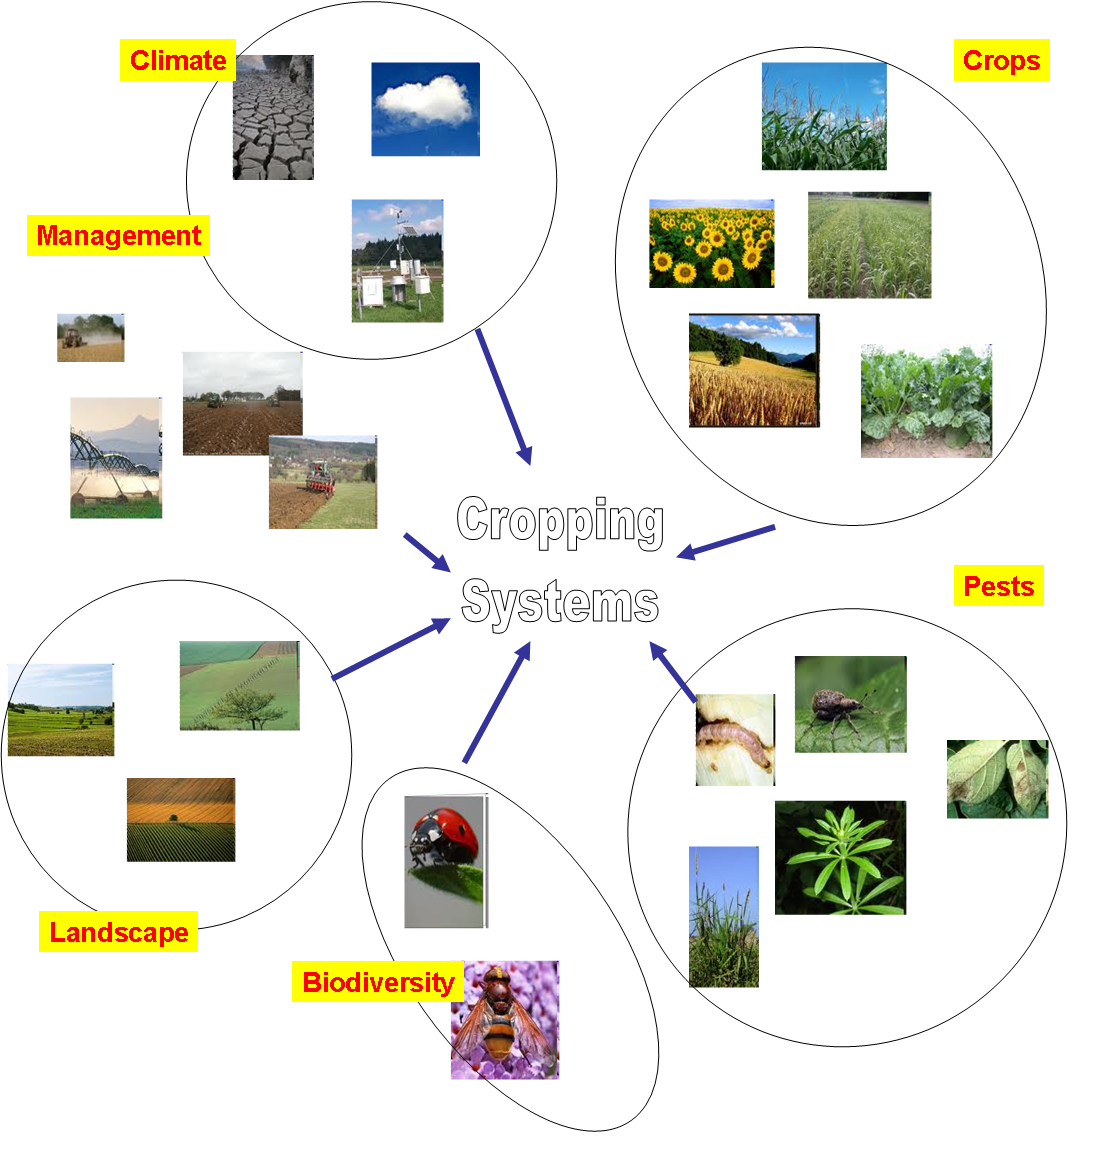
\includegraphics[width=\textwidth]{record}
      %\end{column}
    %\end{columns}
  %\end{figure}
%\end{frame}

\begin{frame}
  \frametitle{Introduction}
  \begin{block}{VLE : Virtual Laboratory Environment}
    \begin{columns}
      \begin{column}{.47\textwidth}
        \begin{itemize}
        \item VLE~\cite{quesnel09} est un environnement de
          multimodélisation et de simulation de systèmes complexes
          dynamiques.
        \item Il est basé sur le formalisme à événements discrets
          \alert{DEVS}~\cite{zeigler00}
        \end{itemize}
        \begin{figure}
          \centering
          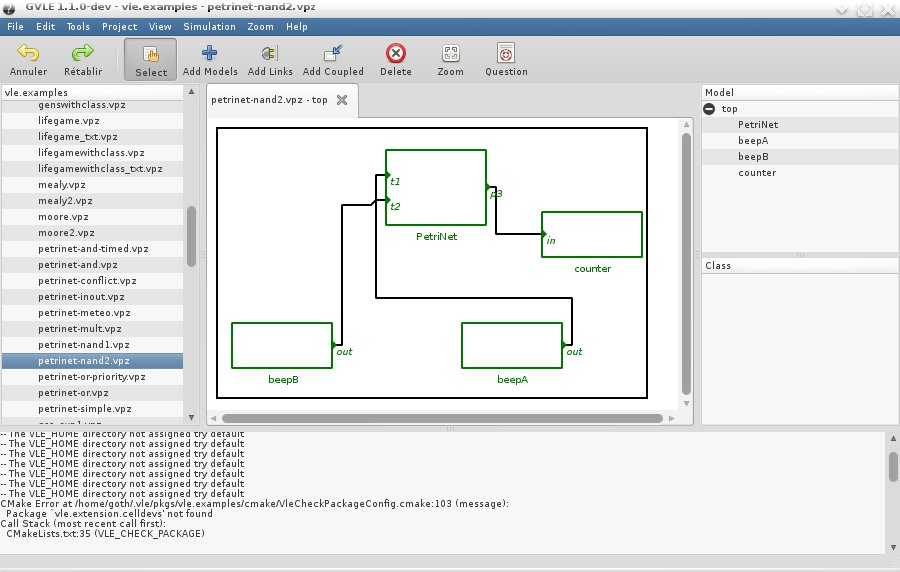
\includegraphics[width=.7\textwidth]{gvle}
        \end{figure}
      \end{column}
      \begin{column}{.47\textwidth}
        \begin{figure}
          \centering
          
\includegraphics[width=.7\textwidth]{yellowvle}
        \end{figure}
        \begin{figure}
          \centering
          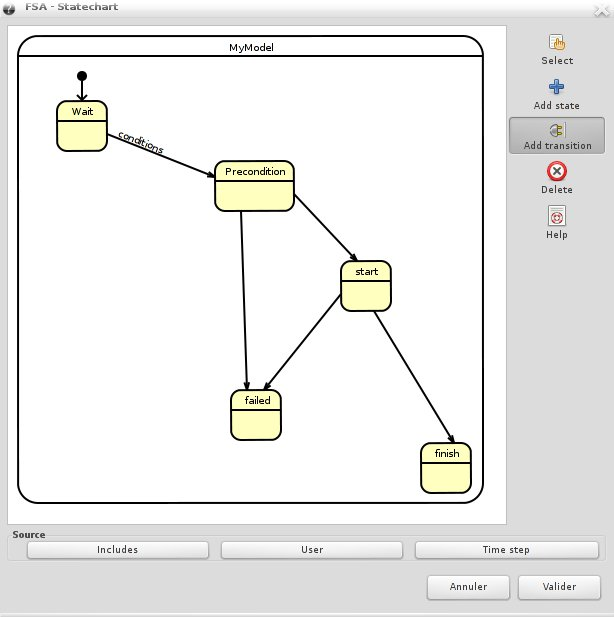
\includegraphics[width=.7\textwidth]{fsa}
        \end{figure}
      \end{column}
    \end{columns}
  \end{block}
\end{frame}

\begin{frame}
  \tableofcontents
\end{frame}

\section{Formalisme DEVS}

\subsection{DEVS}

\begin{frame}
  \frametitle{DEVS}
  \framesubtitle{}
  \begin{exampleblock}{DEVS, un formalisme de M\&S de systèmes
    dynamiques de bas niveau}
    \begin{itemize}
      \item Initié en 1976 par B.\,P.\,Zeigler et est issu des
        \alert{mathématiques discrètes}
    \item Un formalisme à \alert{événements discrets}
    \end{itemize}
    \vfill
     
  \end{exampleblock}
\end{frame}

\begin{frame}
  \frametitle{DEVS}
  \begin{exampleblock}{Simulation de la trajectoire d'une balle}
    \begin{figure}[h]
      \centering
      \includegraphics<1>[width=.7\textwidth]{fig/billard-00}
      \includegraphics<2>[width=.7\textwidth]{fig/billardt-01}
      \includegraphics<3>[width=.7\textwidth]{fig/billardt-02}
      \includegraphics<4>[width=.7\textwidth]{fig/billardt-03}
      \includegraphics<5>[width=.7\textwidth]{fig/billardt-04}
      \includegraphics<6>[width=.7\textwidth]{fig/billardt-05}
      \includegraphics<7>[width=.7\textwidth]{fig/billardt-06}
      \includegraphics<8>[width=.7\textwidth]{fig/billardt-07}
      \includegraphics<9>[width=.7\textwidth]{fig/billarde-08}
      \begin{onlyenv}<2-8>

        Temps discrets : \alert{Quel} est mon état a $t$ ?
      \end{onlyenv}
      \begin{onlyenv}<9>

        Événement discret : \alert{Quand} le prochain changement d'état aura lieu ?
      \end{onlyenv}
    \end{figure}
  \end{exampleblock}
\end{frame}

\begin{frame}
  \frametitle{DEVS}
  \framesubtitle{}
  \begin{exampleblock}{DEVS, un formalisme de M\&S de systèmes
      dynamiques de bas niveau}
    \begin{itemize}
    \item Initié en 1976 par B.\,P.\,Zeigler et est issu des
      \alert{mathématiques discrètes}
    \item Un formalisme à \alert{événements discrets}
    \item Propose deux types de modèles \alert{atomiques} et
      \alert{couplés} :
      \begin{itemize}
      \item les modèles atomiques sont composés d'\alert{états}
        et de fonctions de \alert{transitions} d'états
      \item les modèles couplés proposent une approche
        \alert{modulaire} et \alert{hiérarchique} de la M\&S
      \item possède une propriété importante : un modèle couplé
        possède les mêmes propriétés qu'un modèle atomique
      \end{itemize}
    \item propose un \alert{ensemble d'algorithmes} : les
      simulateurs abstraits
    \end{itemize}
    \pause
    \begin{description}
      \item[Propriété:] les formalismes de systèmes dynamiques
        peuvent être traduits en DEVS
    \end{description}
  \end{exampleblock}
  \pause
  \begin{alertblock}{}
    VLE : Une implémentation des simulateurs abstraits
  \end{alertblock}
\end{frame}

\subsection{Modèle atomique DEVS}

\begin{frame}
  \frametitle{DEVS, Description du modèle atomique}
  \begin{exampleblock}{}
    \begin{columns}
      \begin{column}[c]{.45\textwidth}
        \begin{equation*}
          M = \left\langle X,Y, S, \delta_{\mathit{int}}, \delta_{\mathit{ext}},
            \delta_{\mathit{con}},\lambda, \mathit{ta} \right\rangle
        \end{equation*}
      \end{column}
      \begin{column}[c]{.45\textwidth}
        \begin{figure}[h]
          \begin{center}
            \includegraphics[width=.4\textwidth]{atomic}
          \end{center}
        \end{figure}
      \end{column}
    \end{columns}
  \end{exampleblock}
  \begin{exampleblock}{}
    \begin{itemize}[<+->]
    \item $X$ : l'ensemble des \alert{ports d'entrée} et des valeurs
      attachées
    \item $Y$ : l'ensemble des \alert{ports de sortie} et des valeurs
      attachées
    \item $S$ : l'ensemble des \alert{états} du système
    \item $\delta_{ext}$ : fonction de \alert{transition externe} :
      $\delta_{ext} : S \times X \rightarrow S$\\représente les
      réponses du système aux événements externes
    \item $\delta_{int}$ : fonction de \alert{transition interne} :
      $\delta_{int} : S \rightarrow S$\\représente les évolutions
      autonomes
    \item $\delta_{con}$ : fonction de \alert{conflit} si
      $\delta_{int}$ et $\delta_{ext}$ sont programmées à la même date
    \item $ta(s)$ : \alert{le temps} pendant lequel le modèle reste
      dans l'état $S$. $ta \rightarrow R_0^+$
    \item $\lambda$ : la \alert{fonction de sortie} : $\lambda : S
      \rightarrow Y$ représente les influences externes
    \end{itemize}
  \end{exampleblock}
\end{frame}

\subsection{Modèle couplé DEVS}

\begin{frame}
  \frametitle{DEVS, Description du modèle couplé}
  \begin{exampleblock}{}
    \begin{columns}
      \begin{column}[c]{.45\textwidth}
        \begin{equation*}
          N = \langle X, Y, D, \{M_d\}, \{I_d\}, \{Z_{i,d}\} \rangle
        \end{equation*}
      \end{column}
      \begin{column}{.45\textwidth}
        \begin{figure}[h]
          \begin{center}
            \includegraphics[width=.4\textwidth]{coupled}
          \end{center}
        \end{figure}
      \end{column}
    \end{columns}
  \end{exampleblock}
  \begin{exampleblock}{}
    \begin{itemize}[<+->]
    \item $X$ l'ensemble des \alert{ports d'entrée} et des valeurs
      associées.
    \item $Y$ l'ensemble des \alert{ports de sortie} et des valeurs
      associées.
    \item $D$ l'ensemble des \alert{identifiants des sous modèles}
      avec : $\{ M_d | d \in D \}$.
    \item $\forall d \in D \cup \{N\}$, $I_d$ l'ensemble des perturbateurs de : $d$\\$I_d \subseteq D \cup \{N\},d \notin I_d$
    \item $\forall d \in D \cup \{N\}$\\
      $\forall i \in I_d$, $Z_{i,d}$ est une fonction i-to-d :\\
      \hspace{1cm}$Z_{i,d}:X \rightarrow X_d$, if $i = N$ (connexions d'entrée)\\
      \hspace{1cm}$Z_{i,d}:Y_i \rightarrow Y$, if $d = N$ (connexions de sorties)\\
      \hspace{1cm}$Z_{i,d}:Y_i \rightarrow X_d$ if $i \neq N$ et $d
      \neq N$ (connexions internes)
    \end{itemize}
  \end{exampleblock}
\end{frame}

\subsection{Exemple de dynamique}

\begin{frame}
  \frametitle{DEVS, Dynamique des états}
  \begin{block}{}
    \only<1>{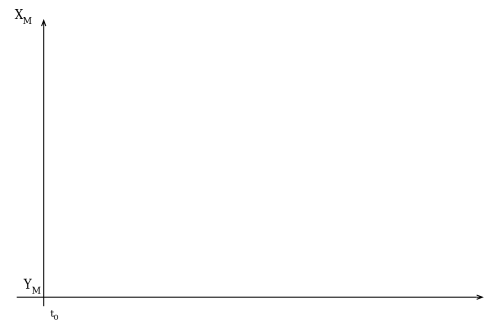
\includegraphics[width=10cm]{exempledevs0}}
    \only<2>{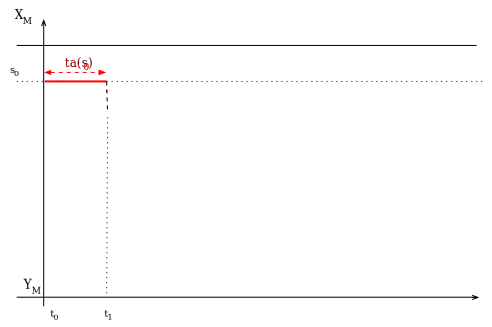
\includegraphics[width=10cm]{exempledevs1}}
    \only<3>{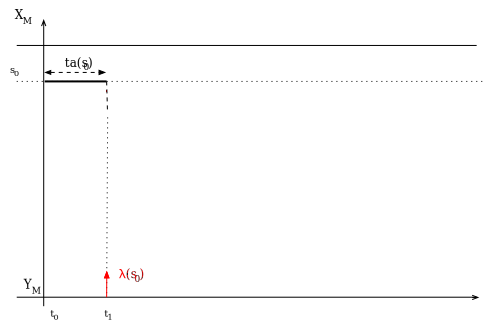
\includegraphics[width=10cm]{exempledevs11}}
    \only<4>{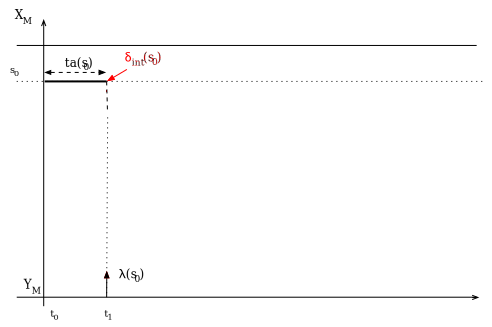
\includegraphics[width=10cm]{exempledevs12}}
    \only<5>{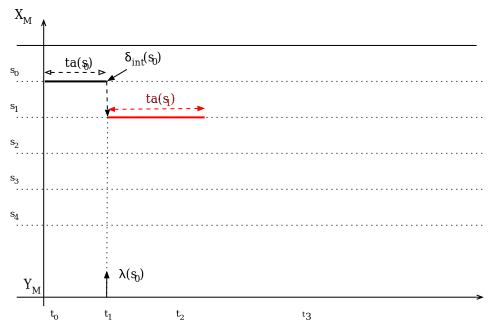
\includegraphics[width=10cm]{exempledevs2}}
    \only<6>{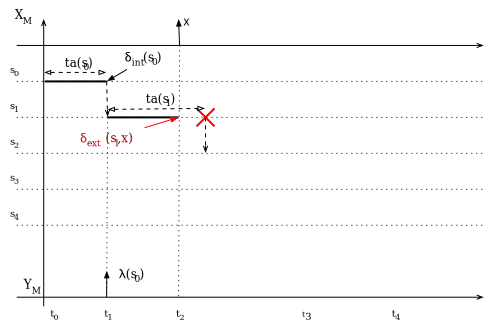
\includegraphics[width=10cm]{exempledevs3}}
    \only<7>{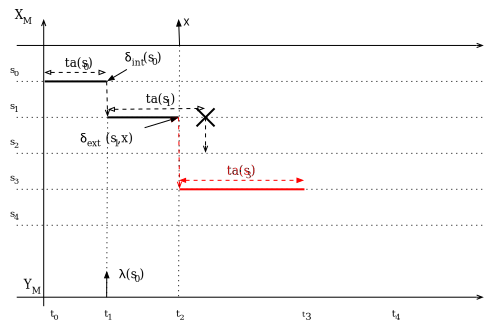
\includegraphics[width=10cm]{exempledevs31}}
  \end{block}
\end{frame}

\subsection{Structure dynamique DEVS}

\begin{frame}
  \frametitle{DEVS, Structure dynamique}
  \begin{exampleblock}{}
    Réseau de modèles : déportent les connexions dans un modèle dit
    \emph{exécutif} :
    \begin{center}
      $DSDEVN_N = \langle X_N, Y_N, \alert{\chi}, \alert{M_{\chi}}
      \rangle$
    \end{center}
  \end{exampleblock}
  \begin{exampleblock}{}
    où :\\
    \begin{itemize}
    \item $X_N$ et $Y_N$ sont les ports d'entrée et de sortie du réseau
    \item $\chi$ le nom du modèle \emph{exécutif}
    \item $M_\chi$ le modèle \emph{exécutif}\\
      \begin{center}
        $M_\chi = \langle X_\chi, Y_\chi, S_\chi, \delta_{int}^\chi,
        \delta_{ext}^\chi, ta_{\chi}, \lambda_{\chi}, \alert{\Sigma^*},
        \alert{\gamma}\rangle$
      \end{center}
      Avec :
      $$\left(
        \begin{array}{l}
          \alert{\gamma} : S_\chi \rightarrow \Sigma^*\text{ la fonction de
            structure}\\
          \alert{\Sigma*} : \text{ l'ensemble des structures}\\
          \Sigma_\alpha \in \Sigma^* :\\
          \hspace{1cm}\Sigma_\alpha = \langle D, EIC, EOC, IC \rangle
        \end{array}
      \right.$$
    \end{itemize}
  \end{exampleblock}
\end{frame}

\section{Projet VLE}

\begin{frame}
  \frametitle{Projet VLE}
  \begin{block}{VLE}
    \begin{itemize}
    \item \alert{Virtual Environment Laboratory}, projet démarré en
      2003,
    \item Environnement de Multimodélisation et de simulation de
      systèmes complexes basé sur DEVS
    \item VLE fournit une bibliothèque C++ appelée VFL
      (\alert{VLE Foundation Library})
    \item VLE fournit un \alert{simulateur en ligne de commande}, une
      \alert{interface graphique} de modélisation, un \alert{paquet R}
      pour l'analyse et la visualisation de résultats, un
      \alert{programme Python} pour le développement de service web et
      un \alert{système de paquets} pour étendre VLE
    \end{itemize}
  \end{block}
  \pause
  \begin{alertblock}{Noyau de simulation}
    \begin{itemize}
    \item Un noyau DSDE (F. Barros) : combine \alert{Parallel DEVS} et
      \alert{Dynamic-Structure DEVS}
    \item Un sous-système d'observation
    \end{itemize}
  \end{alertblock}
\end{frame}

\subsection{Extension d'observation}

\begin{frame}
  \frametitle{VLE, Extension d'observation}
  \begin{columns}[T]
    \begin{column}{.5\textwidth}
      \includegraphics<1->[width=\textwidth]{eto1}

      \includegraphics<2->[width=\textwidth]{eto4}

      \includegraphics<4->[width=\textwidth]{eto3}

      \includegraphics<3->[width=\textwidth]{eto2}
    \end{column}
    \begin{column}{.4\textwidth}
      \begin{block}{}
        \begin{enumerate}
        \item<1-> Montre l'évolution de l'état $S$ d'un système
          dynamique sur $t$
        \item<2-> L'évolution de l'état avec un modèle DEVS (exemple)
        \item<3-> L'observation par pas de temps
        \item<4-> L'observation à la date finale
        \end{enumerate}
      \end{block}
      \begin{alertblock}<3->{} Les points sont les valeurs
        d'observation retournées par la fonction d'observation
        utilisée par $\delta_{\mathit{obs}}$
      \end{alertblock}
    \end{column}
  \end{columns}
\end{frame}

\subsection{Multimodélisation}

\begin{frame}
  \frametitle{Multimodélisation : Définitions}
  \begin{alertblock}{Multimodélisation}
    \begin{itemize}
    \item Un multimodèle est un modèle qui rassemble plusieurs
      paradigmes ou formalismes dans sa réalisation.
      \begin{itemize}
      \item [$\rightarrow$] Augmentation de la puissance descriptive du modèle
      \item [$\rightarrow$] Introduit la notion de couplage
      \end{itemize}
    \item La multimodélisation est l'ensemble des concepts, outils et
      techniques de construction de multimodèles.
    \end{itemize}
  \end{alertblock}
  \begin{block}{Comment coupler des modèles hétérogènes ?}
    \begin{itemize}
    \item Coupler des représentations de la dynamique des sous-systèmes
    \item Intégration des notions de temps, d’espace, d’états et de transition
    \end{itemize}
  \end{block}
  \pause
  \begin{block}{Directions possibles}
    \begin{itemize}
    \item \alert{Co-simulation} : chaque sous modèle a son propre
      simulateur.
    \item La spécification des sous-systèmes dans un \alert{formalisme
        unique} : Réécriture de tous les sous-systèmes dans le même
      formalisme.
    \end{itemize}
  \end{block}
\end{frame}

\begin{frame}
  \frametitle{Multimodélisation : Nos propositions}
  \begin{block}{Sous-formalismes}
    Nous fournissons un ensemble de sous-formalismes développé comme
    des sous-classes du modèle atomic DEVS):\\~\\
    \begin{itemize}
    \item Solvers pour la \alert{simulation d'équations
        différentielles ordinaires d'ordre 1}
      \begin{itemize}
      \item Euler, Runge Kutta order 4, QSS 1 et QSS 2
      \end{itemize}
    \item \alert{Difference equation} (recurrence relation)
    \item \alert{Petri net} (with timed transition, inhibitor arc)
    \item \alert{Finite state automaton}:
      \begin{itemize}
      \item Harel statechart (proche de la spécification des
        statechart UML), Mealy, Moore and FDDEVS
      \end{itemize}
    \item \alert{Decision making} (agent, CSP, planificateur HTN,
      simulation plan, etc).
    \end{itemize}
  \end{block}
\end{frame}

\begin{frame}
  \frametitle{Multimodélisation : Équations aux différences}
  \begin{alertblock}{}
    L'extension \structure{DifferenceEquation} permet de développer des
    modèles à temps discret qui calculent la valeur d'une variable
    réelle en $t$ en fonction d'elle-même à $t-\Delta t$, $t-2\Delta
    t$, \dots{} et en fonction d'autres variables réelles en $t$,
    $t-\Delta t$, $t-2\Delta t$, \dots{}.
  \end{alertblock}
  \begin{block}{Formellement}
    \begin{eqnarray*}
      \forall i \in \{1,\ldots,n\}, &~&\\
      X_i(t)&=&f_i(\underbar Z_i(t),\underbar W_i(t))\\
      \underbar Z_i(t) &=& \begin{bmatrix} X_i(t-\Delta t), \ldots, X_i(0)
      \end{bmatrix}\\
      \underbar W_i(t) &=& \begin{bmatrix} \ldots, \underbar W_{j}(t), \ldots
      \end{bmatrix}\text{ pour } j \in \{1,\ldots,n\}\text{ et }j \neq i\\
      \underbar W_j(t) &=& \begin{bmatrix} X_j(t), X_j(t-\Delta t), \ldots,
        X_j(0) \end{bmatrix}\\
    \end{eqnarray*}
  \end{block}
\end{frame}

\begin{frame}
  \frametitle{Multimodélisation : simulation d'équation
    différentielles du premier ordre}
  \begin{block}{QSS : Quantized State System}
    Méthode proposée par E. Kofman en 2001 pour résoudre des équations
    différentielles du premier ordre basée sur :
    \begin{itemize}
    \item la discrétisation des valeurs au lieu du temps : quantification
    \item le calcul du pas de temps en cohérence avec la pente calculée
      grâce à l'équation
    \item plusieurs algorithmes existent en fonction du degré
      d'approximation (aujourd'hui, il existe QSS1, QSS2 et QSS3)
    \end{itemize}
  \end{block}
  \begin{block}{DESS : Differential Equation System Specification}
    \begin{itemize}
    \item À la différence de QSS, DESS repose sur des schémas
      d'intégration classiques (Euler, Runge Kunta, \ldots) à pas de temps
      d'intégration constant
    \item Les événements de sortie sont produits sur des seuils :
      \begin{itemize}
      \item la variable d'intégration vient de franchir ou est égale à un seuil
      \end{itemize}
    \item Comme QSS, on garde la capacité de perturbation.
    \end{itemize}
  \end{block}
\end{frame}

\begin{frame}
  \frametitle{Multimodélisation : Simulation d'équation
    différentielles du premier ordre}
  \begin{columns}
    \begin{column}{0.48\textwidth}
      \begin{block}{QSS}
        \begin{figure}[h]
          \begin{center}
            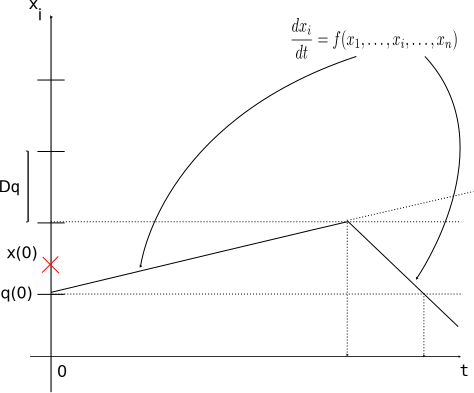
\includegraphics[width=\textwidth]{qss2}
          \end{center}
        \end{figure}
      \end{block}
    \end{column}
    \begin{column}{0.48\textwidth}
      \begin{block}{DESS}
        \begin{figure}[h]
          \begin{center}
            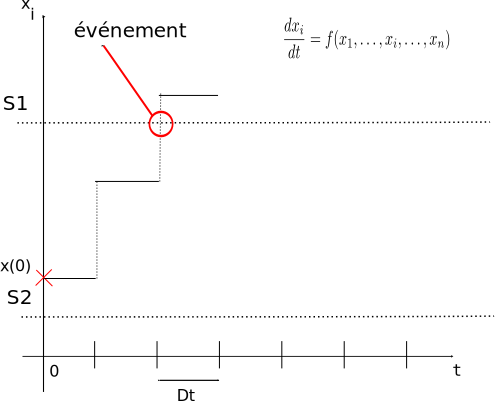
\includegraphics[width=\textwidth]{dess2}
          \end{center}
        \end{figure}
      \end{block}
    \end{column}
  \end{columns}
\end{frame}

\begin{frame}
  \frametitle{Multimodélisation : Réseau de Petri}
  Encapsulation d'un formalisme intemporel comme les réseaux de Petri.
  \tikzstyle{place}=[circle,thick,draw=blue!75,fill=blue!20,minimum size=6mm]
  \tikzstyle{hide place}=[minimum size=6mm]
  \tikzstyle{red place}=[place,draw=red!75,fill=red!20]
  \tikzstyle{transition}=[rectangle,thick,draw=black!75, fill=black!20,minimum
  size=4mm]
  \tikzstyle{every label}=[red]
  \begin{center}
    \begin{tikzpicture}[node distance=1.5cm,>=stealth,bend angle=45,auto]
      \node [hide place] (P0) {};
      \node [hide place] (P00) [right of=P0] {};
      \node [transition] (T1) [above of=P0] {};
      \node [transition] (T2) [below of=P0] {};
      \node [place,tokens=1] (P1) [right of=T1] {};
      \node [place] (P2) [right of=T2] {};
      \node [transition] (T3) [right of=P00] {};
      \node [place,tokens=1] (P3) [right of=T3] {};
      \node [transition] (T4) [right of=P3] {};
      \path[->]
      (T1) edge (P1)
      (T2) edge (P2)
      (P1) edge (T3)
      (P2) edge (T3)
      (T3) edge (P3)
      (P3) edge (T4) ;
      \draw (-1,-2) rectangle (7,2);
      \draw[fill=black] (-1,1.25) -- (-1,1.75) -- (-0.75, 1.5) ;
      \draw[fill=black] (-1,-1.25) -- (-1,-1.75) -- (-0.75, -1.5) ;
      \draw[fill=red] (7,-0.25) -- (7,0.25) -- (7.25, 0) ;
      \path[->,draw=red!75,fill=red!75,dashed]
      (-0.75,1.5) edge (T1)
      (-0.75,-1.5) edge (T2)
      (T4) edge (7,0) ;
    \end{tikzpicture}
  \end{center}
  \begin{alertblock}{À noter}
    Le réseau de Petri possède des extensions temporelle, à priorité,
    stochastique, etc. : \alert{High Level PetriNet}
  \end{alertblock}
\end{frame}

\subsection{Développement de modèles}

\begin{frame}[fragile]
  \frametitle{Développement de modèles}
  \begin{block}{VLE}
    \begin{itemize}
    \item VLE fourni une bibliothèque partagée C++ qui embarque le
      noyau de simulation. Ainsi :
      \begin{itemize}
      \item les utilisateurs doivent développer des classes C++ de
        modèles atomiques, modèles exécutives ou de sous-formalismes
      \end{itemize}
    \end{itemize}
  \end{block}
  \begin{exampleblock}{}
\begin{lstlisting}[language=c++]
class Dynamics
{
public:
  virtual Time timeAdvance() const;

  virtual void internalTransition(const Time& time);

  virtual void externalTransition(const Time& time,
                              const ExternalEventList& lst);
  virtual void output(const Time& time,
                              ExternalEventList& out) const;
  virtual void confluentTransition(const Time& time,
                              const ExternalEventList& lst);
  virtual Value* observation(const ObservationEvent& event) const;
}
\end{lstlisting}
  \end{exampleblock}
\end{frame}

\begin{frame}
  \frametitle{Développement de modèles}
  \begin{block}{Sous-formalismes}
    DEVS permet de développer des sous-formalismes de DEVS\@. Avec VLE
    nous fournissons des extensions :
    \begin{description}
    \item[dynamiques] qui encapsulent un formalisme mathématique comme
      les équations différentielles, réseau de Petri, etc.
    \item[structurelles] qui manipulent la structure du modèle :
      création d'automates cellulaires, des graphes communication, etc.
    \end{description}
  \end{block}
\end{frame}

\begin{frame}[fragile]
  \frametitle{Développement de modèles}
  \begin{block}{Sous formalismes}
    \begin{itemize}
    \item Nous proposons une API simplifiée
    \item Nous proposons des générateurs de code C++
    \end{itemize}
  \end{block}
  \begin{exampleblock}{}
    Par exemple, avec le formalisme des équation aux différences, nous
    fournissons une seule fonction \texttt{compute}. L'api des modèles
    atomiques est cachées.
\begin{lstlisting}
class MyModel: public vle::extension::DifferenceEquation
{
  [...]

  virtual double compute(const Time& time)
  {
    x = y(-1) + z(-1);
    y = z(-1);
  }
};
\end{lstlisting}
  \end{exampleblock}
\end{frame}

\begin{frame}
  \frametitle{Développement de modèles}
  \begin{block}{GVLE : GUI of VLE, un IDE}
    Pour développer des codes sources, la structure du modèle, les
    conditions initiales, les observations, les cadres expérimentaux :
    \begin{figure}[htpb]
      \centering
      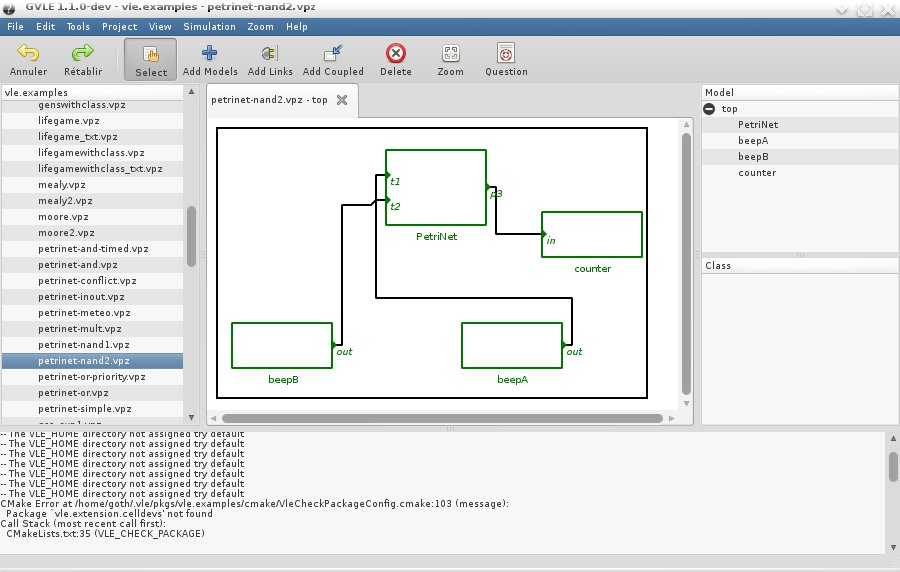
\includegraphics[width=.8\textwidth]{gvle}
    \end{figure}
  \end{block}
\end{frame}

\begin{frame}
  \frametitle{Développement de modèles : exemple}
  \begin{exampleblock}{GUI pour développer un automate}
    \begin{figure}[htpb]
      \centering
      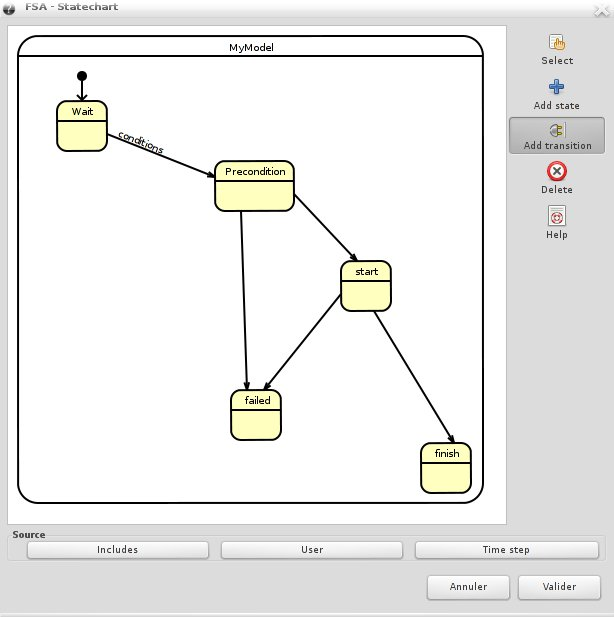
\includegraphics[width=.6\textwidth]{fsa}
    \end{figure}
  \end{exampleblock}
\end{frame}

\begin{frame}
  \frametitle{Développement de modèles : exemple}
  \begin{exampleblock}{Génération de code source}
    \begin{figure}[htpb]
      \centering
      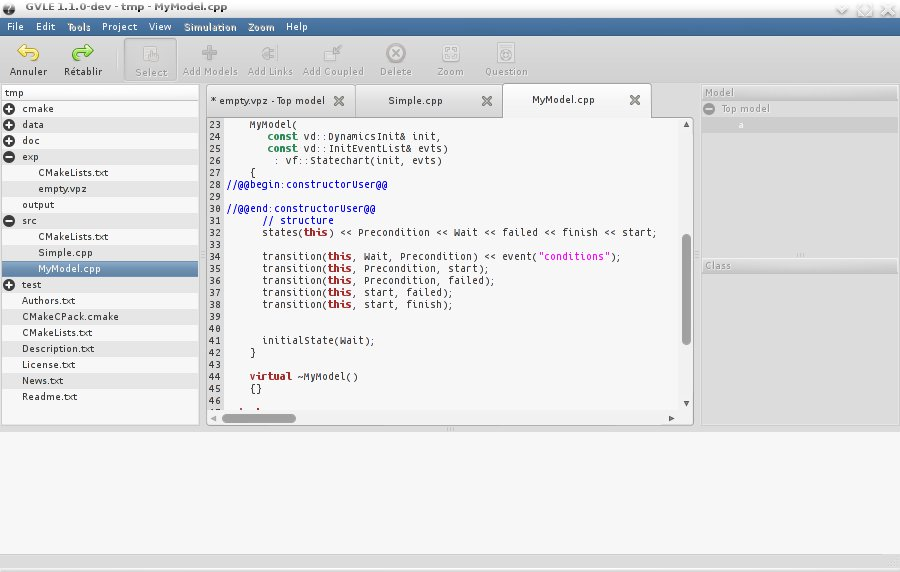
\includegraphics[width=.95\textwidth]{fsa2}
    \end{figure}
  \end{exampleblock}
\end{frame}

\section{Conclusion}

\subsection{Cycle de modélisation}

\begin{frame}
  \frametitle{VLE : Environnement complet de M\&S}
  \framesubtitle{Le cycle de modélisation}
  \begin{center}
    \tikzstyle{action}=[rectangle,draw=OliveGreen!50,fill=OliveGreen!20,thick,
    minimum width=2.5cm, minimum height=1cm]
    \tikzstyle{result}=[rectangle,draw=Mahogany!50,fill=Mahogany!20,thick,
    minimum width=2.5cm, minimum height=1cm]
    \tikzstyle{pre}=[<-,semithick]
    \tikzstyle{post}=[->,semithick]
    \tikzstyle{postr}=[->,thick,draw=Mahogany!50]
    \begin{onlyenv}<1>
      \begin{figure}[htpb]
        \begin{center}
          \includegraphics[width=.7\textwidth]{cycle01}
        \end{center}
      \end{figure}
    \end{onlyenv}
    \begin{onlyenv}<2>
      \begin{figure}[htpb]
        \begin{center}
          \includegraphics[width=.7\textwidth]{cycle02}
        \end{center}
      \end{figure}
    \end{onlyenv}
    \begin{onlyenv}<3>
      \begin{figure}[htpb]
        \begin{center}
          \includegraphics[width=.7\textwidth]{cycle03}
        \end{center}
      \end{figure}
    \end{onlyenv}
    \begin{onlyenv}<4>
      \begin{figure}[htpb]
        \begin{center}
          \includegraphics[width=.7\textwidth]{cycle04}
        \end{center}
      \end{figure}
    \end{onlyenv}
    \begin{onlyenv}<5->
      \begin{figure}[htpb]
        \begin{center}
          \includegraphics[width=.7\textwidth]{cycle05}
        \end{center}
      \end{figure}
    \end{onlyenv}
  \end{center}
  \begin{onlyenv}<1>
    \begin{exampleblock}{}
      \alert{Modélisation} à l'aide des outils
      \alert{classiques} de modélisation, équations
      différentielles, équations aux différences, automates, etc.\ tout
      en restant dans une modélisation de systèmes dynamiques.
    \end{exampleblock}
  \end{onlyenv}
  \begin{onlyenv}<2>
    \begin{exampleblock}{}
      \alert{Implémentation} en code informatique de votre modèle,
      utilisation des \alert{bibliothèques} de \alert{vle} et
      des \alert{extensions proposées} et de l'interface graphique
      \alert{gvle} pour composer vos modèles.
    \end{exampleblock}
  \end{onlyenv}
  \begin{onlyenv}<3>
    \begin{exampleblock}{}
      \alert{Préparer} la plan d'expérience,
      \alert{initialisation} des paramètres et des variables, le
      nombre de \alert{répliquas}, les modèles à
      \alert{observer}, \alert{comment}, et \alert{où} diriger
      les données : \alert{gvle}.
    \end{exampleblock}
  \end{onlyenv}
  \begin{onlyenv}<4>
    \begin{exampleblock}{}
      \alert{Exécute} les simulations depuis \alert{vle},
      \alert{gvle}, \alert{rvle}, \alert{pyvle}, sur une
      machine locale ou une grille de calculs.
    \end{exampleblock}
  \end{onlyenv}
  \begin{onlyenv}<5>
    \begin{exampleblock}{}
      Offrir aux modélisateurs l'accès à DEVS, pour la
      \alert{modélisation} (de modèles hétérogènes), la
      \alert{simulation} (sur grille de calculs), et
      l'\alert{analyse} des sorties, et si possible en proposant
      une \alert{intégration} dans leurs outils.
    \end{exampleblock}
  \end{onlyenv}
\end{frame}

\section{Conclusion}

\begin{frame}
  \frametitle{Conclusion}
  \begin{block}{Vers où ?}
    \begin{itemize}
    \item Plus de formalismes (Multi-agents, équations différentielles
      spatialisées etc.)
    \item Plusieurs noyaux de simulation DEVS spécialisés
      (parallélisation, distribution, hybride temps réel etc.)
    \item Intégrer des travaux de validation
    \item Plus d'IHM
    \item Plus de port (Matlab, Scilab, etc.)
    \end{itemize}
  \end{block}
  \pause
  \begin{block}{Autre projet : PROTEUS}
    \begin{itemize}
      \item «\,Plate-forme pour la Robotique Organisant les Transferts
        Entre Utilisateurs et Scientifiques\,»
      \item Groupe de Recherche en Robotique et partenaires industriels
        (Dassault Aviation, CEA, Thales, LASMEA, INRIA, Onera, etc.
      \item Utilisation de VLE comme simulateur de robot
    \end{itemize}
  \end{block}
\end{frame}

\section*{Références}

\begin{frame}{allowframebreaks}
  \frametitle{Références}
  \small{%
    \bibliographystyle{plain}
    \bibliography{publi}
}
\end{frame}

\end{document}

%%% Local Variables:
%%% coding: utf-8
%%% mode: latex
%%% TeX-engine: xetex
%%% End:
